% This is "sig-alternate.tex" V2.1 April 2013
% This file should be compiled with V2.5 of "sig-alternate.cls" May 2012
%
% This example file demonstrates the use of the 'sig-alternate.cls'
% V2.5 LaTeX2e document class file. It is for those submitting
% articles to ACM Conference Proceedings WHO DO NOT WISH TO
% STRICTLY ADHERE TO THE SIGS (PUBS-BOARD-ENDORSED) STYLE.
% The 'sig-alternate.cls' file will produce a similar-looking,
% albeit, 'tighter' paper resulting in, invariably, fewer pages.
%
% ----------------------------------------------------------------------------------------------------------------
% This .tex file (and associated .cls V2.5) produces:
%       1) The Permission Statement
%       2) The Conference (location) Info information
%       3) The Copyright Line with ACM data
%       4) NO page numbers
%
% as against the acm_proc_article-sp.cls file which
% DOES NOT produce 1) thru' 3) above.
%
% Using 'sig-alternate.cls' you have control, however, from within
% the source .tex file, over both the CopyrightYear
% (defaulted to 200X) and the ACM Copyright Data
% (defaulted to X-XXXXX-XX-X/XX/XX).
% e.g.
% \CopyrightYear{2007} will cause 2007 to appear in the copyright line.
% \crdata{0-12345-67-8/90/12} will cause 0-12345-67-8/90/12 to appear in the copyright line.
%
% ---------------------------------------------------------------------------------------------------------------
% This .tex source is an example which *does* use
% the .bib file (from which the .bbl file % is produced).
% REMEMBER HOWEVER: After having produced the .bbl file,
% and prior to final submission, you *NEED* to 'insert'
% your .bbl file into your source .tex file so as to provide
% ONE 'self-contained' source file.
%
% ================= IF YOU HAVE QUESTIONS =======================
% Questions regarding the SIGS styles, SIGS policies and
% procedures, Conferences etc. should be sent to
% Adrienne Griscti (griscti@acm.org)
%
% Technical questions _only_ to
% Gerald Murray (murray@hq.acm.org)
% ===============================================================
%
% For tracking purposes - this is V2.0 - May 2012

\documentclass{sig-alternate-05-2015}

\usepackage{mathtools}
\begin{document}

% Copyright
%\setcopyright{acmcopyright}
%\setcopyright{acmlicensed}
%\setcopyright{rightsretained}
%\setcopyright{usgov}
%\setcopyright{usgovmixed}
%\setcopyright{cagov}
%\setcopyright{cagovmixed}


%\CopyrightYear{2007} % Allows default copyright year (20XX) to be over-ridden - IF NEED BE.
%\crdata{0-12345-67-8/90/01}  % Allows default copyright data (0-89791-88-6/97/05) to be over-ridden - IF NEED BE.
% --- End of Author Metadata ---

\title {Analysis of the common reccommendation systems with the common frameworks: Spark and Flink}
\subtitle{ Final Report for the BigData project}
%
% You need the command \numberofauthors to handle the 'placement
% and alignment' of the authors beneath the title.
%
% For aesthetic reasons, we recommend 'three authors at a time'
% i.e. three 'name/affiliation blocks' be placed beneath the title.
%
% NOTE: You are NOT restricted in how many 'rows' of
% "name/affiliations" may appear. We just ask that you restrict
% the number of 'columns' to three.
%
% Because of the available 'opening page real-estate'
% we ask you to refrain from putting more than six authors
% (two rows with three columns) beneath the article title.
% More than six makes the first-page appear very cluttered indeed.
%
% Use the \alignauthor commands to handle the names
% and affiliations for an 'aesthetic maximum' of six authors.
% Add names, affiliations, addresses for
% the seventh etc. author(s) as the argument for the
% \additionalauthors command.
% These 'additional authors' will be output/set for you
% without further effort on your part as the last section in
% the body of your article BEFORE References or any Appendices.

\numberofauthors{2} %  in this sample file, there are a *total*
% of EIGHT authors. SIX appear on the 'first-page' (for formatting
% reasons) and the remaining two appear in the \additionalauthors section.
%
\author{
% You can go ahead and credit any number of authors here,
% e.g. one 'row of three' or two rows (consisting of one row of three
% and a second row of one, two or three).
%
% The command \alignauthor (no curly braces needed) should
% precede each author name, affiliation/snail-mail address and
% e-mail address. Additionally, tag each line of
% affiliation/address with \affaddr, and tag the
% e-mail address with \email.
%
% 1st. author
\alignauthor
Mirko Morandi\\
       \affaddr {University of Trento}\\
       \affaddr {176043}\\
       \email {mirko.morandi@unitn.it}\\
% 2nd. author
\alignauthor
Zhiheng Xu\\
        \affaddr {University of Trento}\\
        \affaddr {174222}\\
        \email {zhiheng.xu@unin.it}\\
}

% Just remember to make sure that the TOTAL number of authors
% is the number that will appear on the first page PLUS the
% number that will appear in the \additionalauthors section.

\maketitle
\begin{abstract}

In this paper we provide an extensive analysis of the actual state of the
art of recommendation systems.\\
\textit{Collaborative Filtering} is the current buzzword in the
world of recommendations, came to notoriety after the Netflix Prize
challenge. In this paper we aim to analyze the current implementations
of two different algorithms used for Collaborative Filtering: \textbf{ALS} and \textbf{Stochastic
Gradient Descent} in combination with the common frameworks \texttt{Spark} and  \texttt{Flink}.
\end{abstract}




\keywords{Flink; Spark; CF; Collaborative Filtering; ALS; SGD; Scala}

\section{Introduction}
Recommender systems are now trending due to the overwhelming availability
of data. These systems have the ability to discover hidden relationships between
users and items, and use these patterns to improve the user's taste prediction.
Reserachers discovered a "neighbourhood" of users with a similar taste
which can be revealed by their previous actions: both implicit and explicit.
\texttt{Collaborative filtering} is by far the most common approach adapted also by
some of the biggest companies in the IT sector such as: \textbf{Amazon}, \textbf{Facebook} and \textbf{Netflix}.
Altough it's massive presence in the market \texttt{CF} is not the only approach
available for a recommender system, but it is actually the successor of
\texttt{Content-Based filtering}. The latter aims to profile a user searching
the correlation with the item's peculiarity. By item peculiarity we refer to
its implicit and explicit characteristics, for example a song's genre,
subgenre, writer, composer, year of composition, beats per second etc.
The problem with this approach lays in the difficult of retrieving all the necessary
information, which sometimes are not even available or discloable.
Furthermore with the raise of the BigData paradigm some frameworks started to grow from
the accademic world to the Apache Foundation: \textbf{Flink} and \textbf{Spark}.
Those frameworks can be seen an extension of the Hadoop ecosystem, and both of them
have their own pros and contros which will be briefly analyzed further in this paper.






\section{Collaborative Filtering}

The paper is structured as follow: description in more details
of \texttt{Collaborative Filtering} with it's problems, what are
the most commong algorithms used with \texttt{CF} and a brief
introduction to both \textbf{Flink} and \textbf{Spark}.



\subsection{Collaborative Filtering Approaches}


Collaborative Filtering can be subsenquently defined in two
different approaches:

\subsubsection{Memory-based Content Filtering}
In \texttt{memory-based CF} uses user ratings to compute similarity
between user and items and subsequently make a recommendation. Usually
this approach involves "neighboring" algorithms such as \textbf{K-Nearest Neighbours}
to build relationships between users. The similarity between two users
is calculated using the \textbf{cosine similarity}.\\
\textbf{Cosine similarity} is a measure of similarity between two vectors of an inner product space that measures the cosine of the angle between them.[4]
\begin{equation}
\cos ({\bf t},{\bf e})= {{\bf t} {\bf e} \over \|{\bf t}\| \|{\bf e}\|} = \frac{ \sum_{i=1}^{n}{{\bf t}_i{\bf e}_i} }{ \sqrt{\sum_{i=1}^{n}{({\bf t}_i)^2}} \sqrt{\sum_{i=1}^{n}{({\bf e}_i)^2}} }
\end{equation}
The recommendation is made by finding the top K similar users and aggregate their
user-item matrices to find the appropriate recommendation.
The typical problem of this approach is the difficult with scaling
when the data gets bigger. Due to the \texttt{BigData} paradigm expansion
this approach has been deprecated favoring the following approach.


\subsubsection{Model-based Content Filtering}
The most common approach to \texttt{CF} is through the factorization
of a very big and sparse matrix.[3] For example during the Netflix
Prize at the participans were given a matrix of 8.5 billions of ratings,
of which only 100 millions were non zero values.
\textit{Model-based CF} uses machine-learning and data mining algorithms
to uncover the latent factor model between users and items to
predict the missing ratings.\textbf{latent factor models} are hidden
relationships between users and items hardly discoverable in the original data;
usually they may for example denote the quantity of action in a movie or the complexity
of the characters.These vectors are then used to create the missing values in the user-items
matrix.\\
But what about the error of the prediction? There's an error function better known as %move to section 3
\textbf{Root Mean Square Error} which is used to calculate the difference
between the real and the predicted value.\\
\begin{equation}
{\sqrt {\frac{1} {N}{\sum\limits_{i = 1}^N {(c_{i} - \bar{c}_{i} } })^{2} } }
\end{equation}

Furthermore the model-based content filtering can be expanded in two distinct sections:
\textit{user and item based content filtering} depending on the priority given to the
prediction.


\subsection{Related problems}
\subsubsection{Cold start problem}
Due to the nature of CF, the system needs a huge amount of data
in order to produce a reliable prediction. But what happens if our system
hasn't collected any or not enough information yet?
This problem is called \textbf{cold start} and can be tackled with some advanced
machine learning solutions called \textit{active learning}.

\subsubsection{Shilling Attacks}
CF can be exploited to perturbate its prediction system with a technique
called \textit{shilling attacks}. This happens when the input system (e.g. ratings)
are given in the correct way trying to alter the recommendations to the one
favoured by the attacker. It has also been noticed that these kind of attacks affect
more user-based CF algorithms insted of item-based.[5]

\subsubsection{Sparsity}

In the era of the \textit{web 2.0} the matrices who compose the datasets are
usually very sparse due to the typical proportion for which  \(nUsers \ll nItems\).
As said previously the matrix which was given had only 100M ratings out of
8.5 billions of records. This problem is solved using matrix factorization.


\section{Matrix Factorization}

During the last decade a huge effort has been applied to solve the problem of
big datasets with an incredible amount of data.
Let denote {\large{\textit{\textbf{R}}} = \textit{r{\small ij}}} denote a
user-movie where each element \textit{r{\small ij}} represents a rating given by
a user \textit{i} to an item \textit{j} with a value from 0 to 5; where 0 means
non rated and 1 to 5 a rating ranging relatively from \textit{very poor} to \textit{awesome}.
Let also define \textit{m} the number of users and \textit{n} the number of movies in the system.
The problem of \textit{recommender systems} is to predict the missing values of {\large{\textit{\textbf{R}}}}
using the known ratings.\\
\begin{table}
\centering
\caption{Example of a sparse user-item ratings matrix}
\begin{tabular}{|c|c|c|c|c|c|} \hline
items/users  & \textbf{U1} & \textbf{U2} & \textbf{U3} & \textbf{U4} & \textbf{U5}\\ \hline
\textbf{I1} & 5 & 3 & - & 1 &  3  \\ \hline
\textbf{I2} & 4 & - & 2 & 1 &  -  \\ \hline
\textbf{I3} & 2 & 2 & - & 5 &  - \\ \hline
\textbf{I4} & 4 & 3 & - & 4 &  2  \\ \hline
\textbf{I5} & - & 5 & 5 & 4 &  5  \\ \hline
\end{tabular}
\end{table}
The concept behind \textit{matrix factorization} is to find two matrices
{\large\textit{\textbf{V,W}}} relatively \textit{\textbf{m}} x \textit{\textbf{p}},\textit{\textbf{n}} x \textit{\textbf{p}}. which product
can approximate a much bigger matrix {\large{\textit{\textbf{R}}} of dimensions \textit{\textbf{m}} x \textit{\textbf{n}}.\\
    \textit{R} \(\approx\) \textit{V} * \textit{W}
}\\
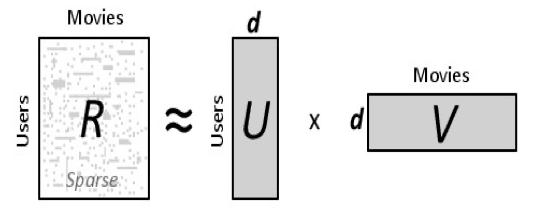
\includegraphics[scale=0.45]{matrix_factorization.png}
The process consists in a low-rank approximation of the user-item matrix using
for both users and items some feature vectors which are used to model
the prediction with a inner vector product of the selected user and item.


\subsection{Tables}
Because tables cannot be split across pages, the best
placement for them is typically the top of the page
nearest their initial cite.  To
ensure this proper ``floating'' placement of tables, use the
environment \textbf{table} to enclose the table's contents and
the table caption.  The contents of the table itself must go
in the \textbf{tabular} environment, to
be aligned properly in rows and columns, with the desired
horizontal and vertical rules.  Again, detailed instructions
on \textbf{tabular} material
is found in the \textit{\LaTeX\ User's Guide}.

Immediately following this sentence is the point at which
Table 1 is included in the input file; compare the
placement of the table here with the table in the printed
dvi output of this document.



To set a wider table, which takes up the whole width of
the page's live area, use the environment
\textbf{table*} to enclose the table's contents and
the table caption.  As with a single-column table, this wide
table will ``float" to a location deemed more desirable.
Immediately following this sentence is the point at which
Table 2 is included in the input file; again, it is
instructive to compare the placement of the
table here with the table in the printed dvi
output of this document.


\begin{table*}
\centering
\caption{Some Typical Commands}
\begin{tabular}{|c|c|l|} \hline
Command&A Number&Comments\\ \hline
\texttt{{\char'134}alignauthor} & 100& Author alignment\\ \hline
\texttt{{\char'134}numberofauthors}& 200& Author enumeration\\ \hline
\texttt{{\char'134}table}& 300 & For tables\\ \hline
\texttt{{\char'134}table*}& 400& For wider tables\\ \hline\end{tabular}
\end{table*}
% end the environment with {table*}, NOTE not {table}!

\subsection{Figures}
Like tables, figures cannot be split across pages; the
best placement for them
is typically the top or the bottom of the page nearest
their initial cite.  To ensure this proper ``floating'' placement
of figures, use the environment
\textbf{figure} to enclose the figure and its caption.

This sample document contains examples of \textbf{.eps} files to be
displayable with \LaTeX.  If you work with pdf\LaTeX, use files in the
\textbf{.pdf} format.  Note that most modern \TeX\ system will convert
\textbf{.eps} to \textbf{.pdf} for you on the fly.  More details on
each of these is found in the \textit{Author's Guide}.


\begin{figure}
\centering
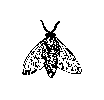
\includegraphics[height=1in, width=1in]{fly}
\caption{A sample black and white graphic
that has been resized with the \texttt{includegraphics} command.}
\end{figure}


As was the case with tables, you may want a figure
that spans two columns.  To do this, and still to
ensure proper ``floating'' placement of tables, use the environment
\textbf{figure*} to enclose the figure and its caption.
and don't forget to end the environment with
{figure*}, not {figure}!

\begin{figure*}
\centering
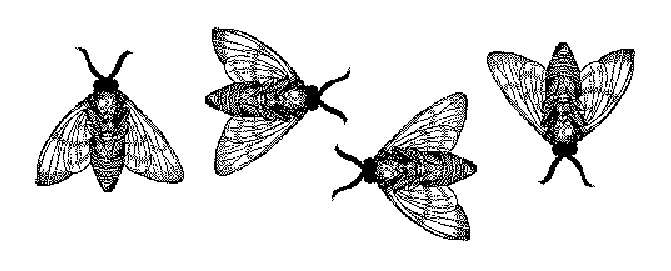
\includegraphics{flies}
\caption{A sample black and white graphic
that needs to span two columns of text.}
\end{figure*}


\begin{figure}
\centering
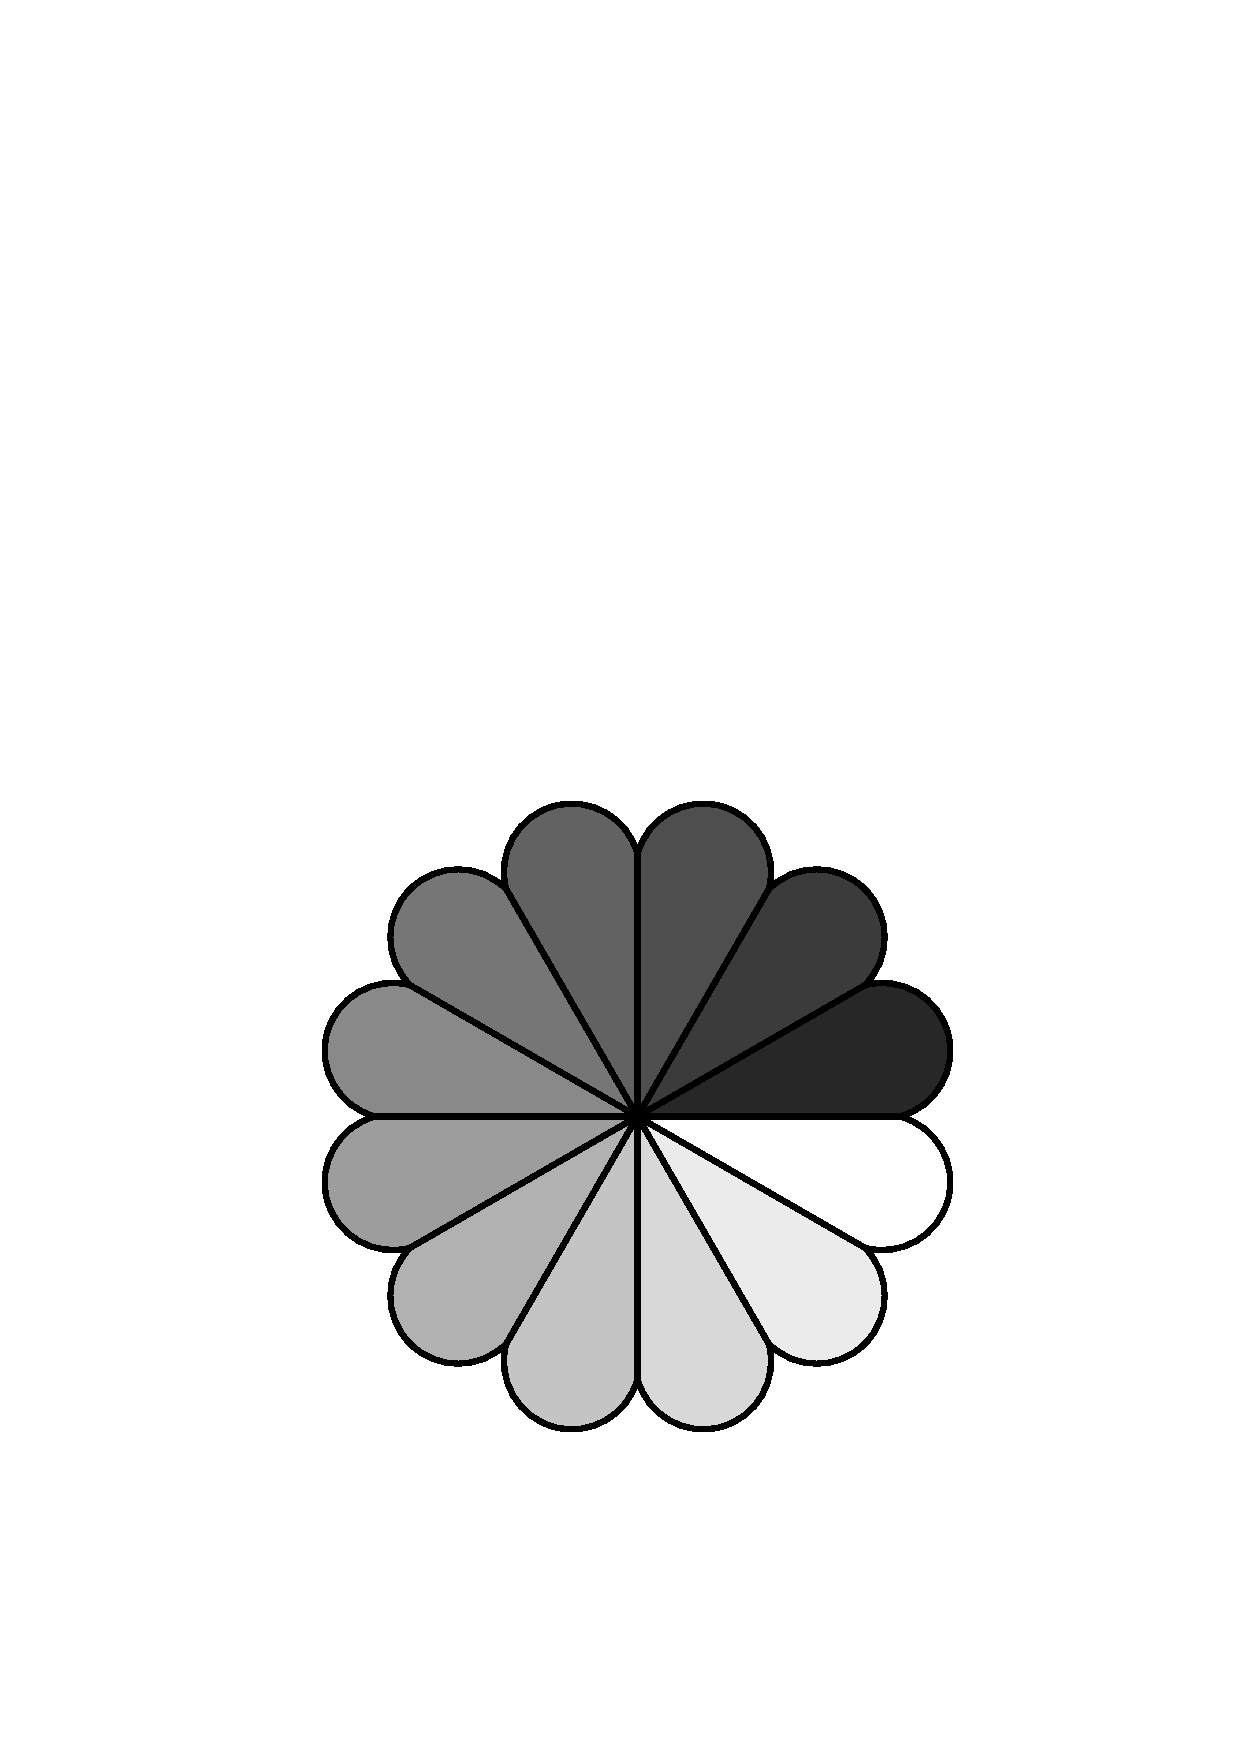
\includegraphics[height=1in, width=1in]{rosette}
\caption{A sample black and white graphic that has
been resized with the \texttt{includegraphics} command.}
\vskip -6pt
\end{figure}

\subsection{Theorem-like Constructs}
Other common constructs that may occur in your article are
the forms for logical constructs like theorems, axioms,
corollaries and proofs.  There are
two forms, one produced by the
command \texttt{{\char'134}newtheorem} and the
other by the command \texttt{{\char'134}newdef}; perhaps
the clearest and easiest way to distinguish them is
to compare the two in the output of this sample document:

This uses the \textbf{theorem} environment, created by
the\linebreak\texttt{{\char'134}newtheorem} command:
\newtheorem{theorem}{Theorem}
\begin{theorem}
Let $f$ be continuous on $[a,b]$.  If $G$ is
an antiderivative for $f$ on $[a,b]$, then
\begin{displaymath}\int^b_af(t)dt = G(b) - G(a).\end{displaymath}
\end{theorem}

The other uses the \textbf{definition} environment, created
by the \texttt{{\char'134}newdef} command:
\newdef{definition}{Definition}
\begin{definition}
If $z$ is irrational, then by $e^z$ we mean the
unique number which has
logarithm $z$: \begin{displaymath}{\log e^z = z}\end{displaymath}
\end{definition}

Two lists of constructs that use one of these
forms is given in the
\textit{Author's  Guidelines}.

There is one other similar construct environment, which is
already set up
for you; i.e. you must \textit{not} use
a \texttt{{\char'134}newdef} command to
create it: the \textbf{proof} environment.  Here
is a example of its use:
\begin{proof}
Suppose on the contrary there exists a real number $L$ such that
\begin{displaymath}
\lim_{x\rightarrow\infty} \frac{f(x)}{g(x)} = L.
\end{displaymath}
Then
\begin{displaymath}
l=\lim_{x\rightarrow c} f(x)
= \lim_{x\rightarrow c}
\left[ g{x} \cdot \frac{f(x)}{g(x)} \right ]
= \lim_{x\rightarrow c} g(x) \cdot \lim_{x\rightarrow c}
\frac{f(x)}{g(x)} = 0\cdot L = 0,
\end{displaymath}
which contradicts our assumption that $l\neq 0$.
\end{proof}

Complete rules about using these environments and using the
two different creation commands are in the
\textit{Author's Guide}; please consult it for more
detailed instructions.  If you need to use another construct,
not listed therein, which you want to have the same
formatting as the Theorem
or the Definition\cite{salas:calculus} shown above,
use the \texttt{{\char'134}newtheorem} or the
\texttt{{\char'134}newdef} command,
respectively, to create it.

\subsection*{A {\secit Caveat} for the \TeX\ Expert}
Because you have just been given permission to
use the \texttt{{\char'134}newdef} command to create a
new form, you might think you can
use \TeX's \texttt{{\char'134}def} to create a
new command: \textit{Please refrain from doing this!}
Remember that your \LaTeX\ source code is primarily intended
to create camera-ready copy, but may be converted
to other forms -- e.g. HTML. If you inadvertently omit
some or all of the \texttt{{\char'134}def}s recompilation will
be, to say the least, problematic.

\section{Conclusions}
This paragraph will end the body of this sample document.
Remember that you might still have Acknowledgments or
Appendices; brief samples of these
follow.  There is still the Bibliography to deal with; and
we will make a disclaimer about that here: with the exception
of the reference to the \LaTeX\ book, the citations in
this paper are to articles which have nothing to
do with the present subject and are used as
examples only.
%\end{document}  % This is where a 'short' article might terminate

%ACKNOWLEDGMENTS are optional
\section{Acknowledgments}
This section is optional; it is a location for you
to acknowledge grants, funding, editing assistance and
what have you.  In the present case, for example, the
authors would like to thank Gerald Murray of ACM for
his help in codifying this \textit{Author's Guide}
and the \textbf{.cls} and \textbf{.tex} files that it describes.

%
% The following two commands are all you need in the
% initial runs of your .tex file to
% produce the bibliography for the citations in your paper.
\bibliographystyle{abbrv}
\bibliography{sigproc}  % sigproc.bib is the name of the Bibliography in this case
% You must have a proper ".bib" file
%  and remember to run:
% latex bibtex latex latex
% to resolve all references
%
% ACM needs 'a single self-contained file'!
%
%APPENDICES are optional
%\balancecolumns
\appendix
%Appendix A
\section{Headings in Appendices}
The rules about hierarchical headings discussed above for
the body of the article are different in the appendices.
In the \textbf{appendix} environment, the command
\textbf{section} is used to
indicate the start of each Appendix, with alphabetic order
designation (i.e. the first is A, the second B, etc.) and
a title (if you include one).  So, if you need
hierarchical structure
\textit{within} an Appendix, start with \textbf{subsection} as the
highest level. Here is an outline of the body of this
document in Appendix-appropriate form:
\subsection{Introduction}
\subsection{The Body of the Paper}
\subsubsection{Type Changes and  Special Characters}
\subsubsection{Math Equations}
\paragraph{Inline (In-text) Equations}
\paragraph{Display Equations}
\subsubsection{Citations}
\subsubsection{Tables}
\subsubsection{Figures}
\subsubsection{Theorem-like Constructs}
\subsubsection*{A Caveat for the \TeX\ Expert}
\subsection{Conclusions}
\subsection{Acknowledgments}
\subsection{Additional Authors}
This section is inserted by \LaTeX; you do not insert it.
You just add the names and information in the
\texttt{{\char'134}additionalauthors} command at the start
of the document.
\subsection{References}
Generated by bibtex from your ~.bib file.  Run latex,
then bibtex, then latex twice (to resolve references)
to create the ~.bbl file.  Insert that ~.bbl file into
the .tex source file and comment out
the command \texttt{{\char'134}thebibliography}.
% This next section command marks the start of
% Appendix B, and does not continue the present hierarchy
\section{More Help for the Hardy}
The sig-alternate.cls file itself is chock-full of succinct
and helpful comments.  If you consider yourself a moderately
experienced to expert user of \LaTeX, you may find reading
it useful but please remember not to change it.
%\balancecolumns % GM June 2007
% That's all folks!
\end{document}
